\documentclass[hyperref=unicode,presentation,10pt]{beamer}

\usepackage[absolute,overlay]{textpos}
\usepackage{array}
\usepackage{graphicx}
\usepackage{adjustbox}
\usepackage[version=4]{mhchem}
\usepackage{chemfig}
\usepackage{caption}
\usepackage{makecell}

%dělení slov
\usepackage{ragged2e}
\let\raggedright=\RaggedRight
%konec dělení slov

\addtobeamertemplate{frametitle}{
	\let\insertframetitle\insertsectionhead}{}
\addtobeamertemplate{frametitle}{
	\let\insertframesubtitle\insertsubsectionhead}{}

\makeatletter
\CheckCommand*\beamer@checkframetitle{\@ifnextchar\bgroup\beamer@inlineframetitle{}}
\renewcommand*\beamer@checkframetitle{\global\let\beamer@frametitle\relax\@ifnextchar\bgroup\beamer@inlineframetitle{}}
\makeatother
\setbeamercolor{section in toc}{fg=red}
\setbeamertemplate{section in toc shaded}[default][100]

\usepackage{fontspec}
\usepackage{unicode-math}

\usepackage{polyglossia}
\setdefaultlanguage{czech}

\def\uv#1{„#1“}

\mode<presentation>{\usetheme{default}}
\usecolortheme{crane}

\setbeamertemplate{footline}[frame number]

\title[Crisis]
{C2062 -- Anorganická chemie II}

\subtitle{Ruthenium, rhodium a palladium}
\author{Zdeněk Moravec, hugo@chemi.muni.cz \\ \adjincludegraphics[height=60mm]{img/IUPAC_PSP.jpg}}
\date{}

\begin{document}

\begin{frame}
	\titlepage
\end{frame}

\section{Úvod}
\frame{
	\frametitle{}
	\vfill
	\begin{figure}
		\adjincludegraphics[width=\textwidth]{img/Periodic_table_AH.png}
	\end{figure}
	\vfill
}

\frame{
	\frametitle{}
	\vfill
	\textbf{Platinové kovy}
	\begin{itemize}
		\item Ru, Rh, Pd, Os, Ir a Pt
		\item Patří k nejvzácnějším prvkům na Zemi.\footnote[frame]{\href{https://is.muni.cz/do/sci/UChem/um/spchp/ch27s01.html}{Platinové kovy}}
		\item \textit{Lehké platinové kovy} mají hustotu okolo 12~g.cm$^{-3}$: Ru, Rh a Pd.
		\item \textit{Těžké platinové kovy} mají hustotu okolo 22~g.cm$^{-3}$: Os, Ir a Pt.
		\item Jejich výroba je vždy spojena s výrobou jiného kovu, protože jsou příměsí rud.
	\end{itemize}
	\begin{center}
	\begin{tabular}{|l|l|l|l|}
		\hline
		\textbf{Lehké platinové kovy} & Ru & Rh & Pd \\\hline
		Hustota {[g.cm$^{-3}$]} & 12,41 & 12,41 & 12,02 \\\hline
		\textbf{Těžké platinové kovy} & Os & Ir & Pt \\\hline
		Hustota {[g.cm$^{-3}$]} & 22,59 & 22,56 & 21,45 \\\hline
	\end{tabular}
	\end{center}
	\vfill
}

\frame{
	\frametitle{}
	\vfill
	\begin{tabular}{|c|l|l|l|}
	\hline
	 & \textit{Ruthenium} & \textit{Rhodium} & \textit{Palladium} \\\hline
	 El. konfigurace & 4d$^{7}$ 5s$^{1}$ & 4d$^{8}$ 5s$^{1}$ & 4d$^{10}$ \\\hline
	 Teplota tání [$^\circ$C] & 2334 & 1964 & 1555 \\\hline
	 Teplota varu [$^\circ$C]  & 4150 & 3695 & 2963 \\\hline
	 Objeven & 1844 & 1804 & 1802 \\\hline
	 Vzhled & stříbrno-bílý\footnote[frame]{Zdroj: \href{https://commons.wikimedia.org/wiki/File:Ruthenium_a_half_bar.jpg}{Alchemist-hp/Commons}} & stříbrno-bílý\footnote[frame]{Zdroj: \href{https://commons.wikimedia.org/wiki/File:Rhodium_powder_pressed_melted.jpg}{Alchemist-hp/Commons}} & stříbrno-bílý\footnote[frame]{Zdroj: \href{https://commons.wikimedia.org/wiki/File:Palladium.jpg}{Jurii/Commons}} \\
	 &  \begin{minipage}{.2\textwidth}
	 	\adjincludegraphics[width=\linewidth]{img/Ruthenium.jpg}
	 \end{minipage}
	 	& \begin{minipage}{.2\textwidth}
	 		\adjincludegraphics[width=\linewidth]{img/Rhodium.jpg}
	 	\end{minipage} & \begin{minipage}{.2\textwidth}
	 	\adjincludegraphics[width=\linewidth]{img/Palladium.jpg}
 	\end{minipage} \\\hline
	\end{tabular}
	\vfill
}

\section{Chemické a fyzikální vlastnosti}
\subsection{Ušlechtilé a neušlechtilé kovy}
\frame{
	\frametitle{}
	\begin{columns}

		\column{.5\textwidth}
		\begin{tabular}{|l|r@{,}l|}
			\hline
			\textbf{Elektroda} & \multicolumn{2}{|c|}{\textbf{E$^0$ [V]}} \\\hline
			Li/Li$^+$ & -3 & 045 \\\hline
			Cs/Cs$^+$ & -3 & 026 \\\hline
			Rb/Rb$^+$ & -2 & 98 \\\hline
			K/K$^+$ & -2 & 931 \\\hline
			Ba/Ba$^{2+}$ & -2 & 912 \\\hline
			Sr/Sr$^{2+}$ & -2 & 899 \\\hline
			Na/Na$^+$ & -2 & 714 \\\hline
			Mg/Mg$^{2+}$ & -2 & 363 \\\hline
			Al/Al$^{3+}$ & -1 & 66 \\\hline
			Zn/Zn$^{2+}$ & -0 & 762 \\\hline
			Fe/Fe$^{2+}$ & -0 & 440 \\\hline
			Co/Co$^{2+}$ & -0 & 277 \\\hline
			Ni/Ni$^{2+}$ & -0 & 250 \\\hline
			\textbf{H/H$^+$} & \textbf{0} & \textbf{000} \\\hline
		\end{tabular}

		\column{.5\textwidth}
		\begin{tabular}{|l|r@{,}l|}
			\hline
			\textbf{Elektroda} & \multicolumn{2}{|c|}{\textbf{E$^0$ [V]}} \\\hline
			Bi/Bi$^{3+}$ & 0 & 200 \\\hline
			Ru/Ru$^{2+}$ & 0 & 300 \\\hline
			Cu/Cu$^{2+}$ & 0 & 337 \\\hline
			Cu/Cu$^+$ & 0 & 521 \\\hline
			W/W$^{6+}$ & 0 & 68 \\\hline
			Os/Os$^{2+}$ & 0 & 69 \\\hline
			Ag/Ag$^+$ & 0 & 799 \\\hline
			Pb/Pb$^{4+}$ & 0 & 800 \\\hline
			Hg/Hg$^{2+}$ & 0 & 851 \\\hline
			Ir/Ir$^{3+}$ & 1 & 16 \\\hline
			Pt/Pt$^{2+}$ & 1 & 200 \\\hline
			Au/Au$^{3+}$ & 1 & 498 \\\hline
			Au/Au$^{+}$ & 1 & 691 \\\hline
		\end{tabular}
	\end{columns}
}

\frame{
	\frametitle{}
	\begin{columns}
		\begin{column}{.65\textwidth}
			\begin{itemize}
				\item Čím má kov negativnější potenciál, tím se snadněji oxiduje a má silnější redukční schopnosti.
				\item Cu/Cu$^{2+}$: 0,337 V
				\item Fe/Fe$^{2+}$: $-$0,440 V
				\item \ce{Cu + FeSO4 -> CuSO4 + Fe}
				\begin{itemize}
					\item Měd má kladnější potenciál a proto reakce \textit{nepoběží samovolně}.
				\end{itemize}
				\item \ce{Fe + CuSO4 -> FeSO4 + Cu}
				\begin{itemize}
					\item Železo má zápornější potenciál a proto reakce \textit{poběží samovolně}.
					\item Železný drát ponořený do roztoku modré skalice se po chvíli začne pokrývat vyloučenou mědí.
				\end{itemize}
			\end{itemize}
		\end{column}
		\begin{column}{.35\textwidth}
			\begin{figure}
				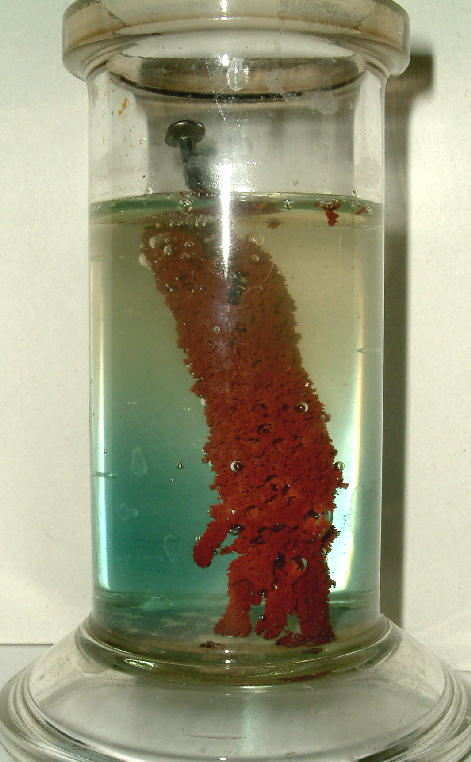
\includegraphics[keepaspectratio,height=.6\textheight]{img/Fe-nagel_in_CuSO4.jpg}
				\caption*{Železo v roztoku modré skalice.\footnote[frame]{Zdroj: \href{https://commons.wikimedia.org/wiki/File:Fe-nagel_in_CuSO4.jpg}{H. Hoffmeister/Commons}}}
			\end{figure}
		\end{column}
	\end{columns}
}

\subsection{Ruthenium}
\frame{
	\frametitle{}
	\vfill
	\textbf{Ruthenium}
	\begin{itemize}
		\item Krystaluje v nejtěsnějším hexagonálním uspořádání.
		\item Má sedm stabilních izotopů a 27 radioizotopů.
		\begin{itemize}
			\item \ce{^{96}Ru}; 5,54~\%
			\item \ce{^{98}Ru}; 1,87~\%
			\item \ce{^{99}Ru}; 12,76~\% -- využívá se v NMR spektroskopii (I = $\frac{3}{2}$)\footnote[frame]{\href{https://doi.org/10.1021/om990477n}{$^{99}$Ru NMR Spectroscopy of Organometallic and Coordination Complexes of Ruthenium(II)}}
			\item \ce{^{100}Ru}; 12,60~\%
			\item \ce{^{101}Ru}; 17,06~\%
			\item \ce{^{102}Ru}; 31,55~\%
			\item \ce{^{104}Ru}; 18,62~\%
		\end{itemize}
		\item Na vzduchu je stálé.
		\item Vytváří sloučeniny v rozmezí oxidačních čísel $-$II až VIII.
		\item Běžné oxidační stavy jsou II, III a IV.
		\item Důležitou sloučeninou je černý chlorid ruthenitý, \ce{RuCl3}, který je výchozí látkou pro syntézu sloučenin ruthenia.
	\end{itemize}
	\vfill
}

\subsection{Rhodium}
\frame{
	\frametitle{}
	\vfill
	\textbf{Rhodium}
	\begin{columns}
		\begin{column}{.7\textwidth}
		\begin{itemize}
			\item Krystaluje v nejtěsnějším hexagonálním uspořádání.
			\item Má jeden stabilní izotop \ce{^{103}Rh} a 33 radioizotopů.
			\item Jeho elektronová konfigurace je {[Kr]} 4d$^8$ 5s$^1$.
			\item Na vzduchu je stálé, je velice odolné vůči působení kyselin, vč. lučavky královské.
			\item Za červeného žáru reaguje pomalu s kyslíkem a halogeny.
			\item Vytváří sloučeniny v rozmezí oxidačních čísel 0~až~VI.
			\item Běžným a nejstabilnějším oxidačním stavem je III.
		\end{itemize}
		\end{column}
		\begin{column}{.3\textwidth}
			\begin{tabular}{|l|l|}
				\hline
				0 & \ce{Rh4(CO)12} \\\hline
				1 & \ce{RhCl(PH3)2} \\\hline
				2 & \ce{Rh2(O2CCH3)4} \\\hline
				3 & \ce{RhCl3}, \ce{Rh2O3} \\\hline
				4 & \ce{RhO2} \\\hline
				5 & \ce{RhF5}, \ce{Sr3LiRhO6} \\\hline
				6 & \ce{RhF6} \\\hline
			\end{tabular}

			\begin{figure}
				\adjincludegraphics[width=.9\textwidth]{img/Rh4_CO_12.png}
				\caption*{\ce{Rh4(CO)12}}
			\end{figure}
		\end{column}
	\end{columns}
	\vfill
}

\subsection{Palladium}
\frame{
	\frametitle{}
	\vfill
	\textbf{Palladium}
	\begin{itemize}
		\item Palladium krystaluje v plošně centrované kubické mřížce (fcc).
		\item Přírodní palladium se skládá ze šesti stabilních izotopů a jednoho nestabilního. Dále známe 23 radioizotopů.
		\begin{itemize}
			\item \ce{^{102}Pd}; 1,02~\%
			\item \ce{^{104}Pd}; 11,14~\%
			\item \ce{^{105}Pd}; 22,33~\%
			\item \ce{^{106}Pd}; 27,33~\%
			\item \ce{^{107}Pd}; stopová množství; 6,5$\times$10$^6$ let
			\item \ce{^{108}Pd}; 26,46~\%
			\item \ce{^{110}Pd}; 11,72~\%
		\end{itemize}
		\item Palladium se rozpouští v horké kyselině dusičné i lučavce královské.
		\item Reaguje s taveninami alkalických hydroxidů.
	\end{itemize}
	\vfill
}

\frame{
	\frametitle{}
	\vfill
	\begin{itemize}
		\item Běžná oxidační čísla jsou II a IV, oxidační stav IV je ale stabilnější u platiny.
		\item V oxidačním čísle IV známe řadu komplexů s halogenidy, \ce{[PdX6]^{2-}}.
		\item Hexachloropalladičité komplexy, \ce{[PdCl6]^{2-}}, lze získat rozpouštěním palladia v lučavce královské.
		\item Komplexy v oxidačním čísle II mají čtvercovou geometrii a jsou diamagnetické (nízkospinové).
		\item Je reaktivnější než platina, za vysokých teplot reaguje s kyslíkem, fluorem a chlorem.
		\item \ce{PdO <-[O2, 350 $^\circ$C] Pd ->[Cl2, 500 $^\circ$C] PdCl2}
	\end{itemize}
	\begin{figure}
		\adjincludegraphics[width=.75\textwidth]{img/Alpha-PdCl2.png}
		\caption*{Krystalová struktura \ce{$\alpha$-PdCl2}.\footnote[frame]{Zdroj: \href{https://commons.wikimedia.org/wiki/File:Alpha-palladium(II)-chloride-chain-from-xtal-3D-balls.png}{CCoil/Commons}}}
	\end{figure}
	\vfill
}

\section{Výskyt a získávání}
\subsection{Ruthenium}
\frame{
	\frametitle{}
	\vfill
	\begin{itemize}
		\item Ruthenium je velmi vzácné, jeho koncentrace v zemské kůře je jen 100~ppt.
		\item Vyskytuje se společně s dalšími platinovými kovy.
		\item Komerčně významná množství se nacházejí i v minerálu pentlanditu\footnote[frame]{\href{https://mineraly.sci.muni.cz/sulfidy/pentlandit.html}{Pentlandit}} (\ce{(Fe,Ni)9S8}) a v pyroxenitech.\footnote[frame]{\href{http://geologie.vsb.cz/PETROLOGIE2013/klasifikace-hh-pyroxenity.htm}{Pyroxenity}}
		\item V roce 2020 byla roční produkce ruthenia v USA 11 tun.\footnote[frame]{\href{https://pubs.usgs.gov/periodicals/mcs2021/mcs2021-platinum.pdf}{Platinum-group metals}}
		\item Světové zásoby jsou odhadovány na 5 000 tun.
		\item Stejně jako jiné platinové kovy se získává ruthenium jako vedlejší produkt výroby niklu a mědi.
		\item Během elektrolytického čištění přecházejí platinové kovy do anodových kalů.
		\item Kovy jsou převáděny do roztoku, nejpoužívanější metoda je mineralizace pomocí peroxidu sodného (\ce{Na2O2}).
	\end{itemize}
	\vfill
}

\frame{
	\frametitle{}
	\vfill
	\begin{itemize}
		\item Produkt mineralizace se rozpustí v lučavce královské.
		\item Ru, Os, Rh a Ir zůstávají nerozpuštěny a jsou separovány.
		\item Rhodium se získá reakcí s taveninou hydrogensíranu sodného.
		\item Zbylá pevná fáze je rozpuštěna reakcí s oxidem sodným, \ce{Na2O}, čímž se získá roztok obsahující Ru a Os a pevná látka obsahující iridium.
		\item Oba kovy jsou oxidovány na \ce{MO4} a separovány destilací, extrakcí nebo srážením \ce{(NH4)3RuCl6}.\footnote[frame]{\href{https://doi.org/10.1021/cr60103a002}{The Platinum Metals.}}
		\item Kovové ruthenium je získáno redukcí vodíkem.
	\end{itemize}
	\vfill
}

\subsection{Rhodium}
\frame{
	\frametitle{}
	\vfill
	\begin{itemize}
		\item Koncentrace rhodia v zemské kůře je jen okolo 0,2~ppb.
		\item Koncentrace v meteoritech je vyšší, přibližně 1~ppb.
		\item Vyskytuje se společně s dalšími platinovými kovy.
		\item Komerčně se získává z platinových rud.
		\item Roční celosvětová produkce se pohybuje pod 30 tun, hlavními producenty jsou Jižní Afrika a Rusko.\footnote[frame]{\href{https://d9-wret.s3.us-west-2.amazonaws.com/assets/palladium/production/atoms/files/myb1-2018-plati.pdf}{2018 Minerals Yearbook}}
	\end{itemize}
	\begin{figure}
		\adjincludegraphics[height=.35\textheight]{img/Rh_price.png}
		\caption*{Vývoj ceny kovového rhodia.\footnote[frame]{Zdroj: \href{https://commons.wikimedia.org/wiki/File:Rh_price.png}{Materialscientist/Commons}}}
	\end{figure}
	\vfill
}

\subsection{Palladium}
\frame{
	\frametitle{}
	\vfill
	\begin{itemize}
		\item Koncentrace palladia v zemské kůře je jen okolo 15~ppb.
		\item V přírodě se nachází i v ryzím stavu ve formě slitin se zlatem a platinovými kovy.
		\item Hlavním průmyslovým zdrojem jsou rudy niklu a mědi.
		\item Celosvětová produkce palladia do roku 2016 byla 208 tun.
		\item Hlavními výrobci jsou Rusko a Jižní Afrika.
		\item Lze ho získat i z vyhořelého jaderného paliva.\footnote[frame]{\href{https://doi.org/10.1134/S106636222203002X}{Prospects for the Use of Palladium from NPP Spent Nuclear Fuel and Ways to Design the Technology of its Recovery at a Radiochemical Enterprise}}
	\end{itemize}
	\vfill
}

\section{Využití}
\subsection{Ruthenium}
\frame{
	\frametitle{}
	\vfill
	\begin{itemize}
		\item Hlavní využití nachází ruthenium v elektronice a katalýze.
		\item V elektronice se ruthenium používá např. pro konstrukci kondenzátorů MIM (Metal-Insulator-Metal) v nových typech DRAM pamětí.\footnote[frame]{\href{https://research.tue.nl/en/studentTheses/atomic-layer-deposition-of-ruthenium-thin-films-using-oxygen}{Atomic layer deposition of Ruthenium thin films using oxygen}}
		\item Také se slévá s platinou a palladiem, protože zlepšuje jejich vlastnosti.
	\end{itemize}
	\begin{figure}
		\adjincludegraphics[width=.6\textwidth]{img/DDR4_Ram.jpg}
		\caption*{RAM modul.\footnote[frame]{Zdroj: \href{https://commons.wikimedia.org/wiki/File:DDR4_Ram_IMGP5859_smial_wp.jpg}{Smial/Commons}}}
	\end{figure}
	\vfill
}

\frame{
	\frametitle{}
	\vfill
	\begin{itemize}
		\item Roztoky chloridu ruthenitého, \ce{RuCl3}, jsou velmi účinné katalyzátory pro metathezi olefinů a hydrogenační reakce.
	\end{itemize}
	\begin{figure}
		\adjincludegraphics[width=\textwidth]{img/Polynbornene.png}
	\end{figure}
	\begin{figure}
		\adjincludegraphics[width=\textwidth]{img/RuCl-catalysed.png}
	\end{figure}
	\vfill
}

\subsection{Rhodium}
\frame{
	\frametitle{}
	\vfill
	\begin{itemize}
		\item Hlavní využití rhodia je v katalýze.
		\item Využívá se jako katalyzátor (trojčinný, nesprávně třícestý) v automobilech, kde zajišťuje rozklad oxidů dusíku, oxidaci CO a uhlovodíků:\footnote[frame]{\href{https://doi.org/10.1080/01614949408009468}{Why Rhodium in Automotive Three-Way Catalysts?}}
		\item \ce{2 NOx -> x O2 + N2}
		\item \ce{2 CO + O2 -> 2 CO2}
		\item Dále katalyzuje velké množství průmyslových procesů, např. výrobu kyseliny octová (viz další strana).
	\end{itemize}
	\begin{figure}
		\adjincludegraphics[height=.25\textheight]{img/Katalysator_fur_Auto.jpg}
		\caption*{Automobilový katalyzátor.\footnote[frame]{Zdroj: \href{https://commons.wikimedia.org/wiki/File:Aufgeschnittener_Metall_Katalysator_für_ein_Auto.jpg}{Stahlkocher/Commons}}}
	\end{figure}
	\vfill
}

\frame{
	\frametitle{}
	\vfill
	\textbf{Monsanto proces}
	\begin{itemize}
		\item Průmyslová metoda výroby kyseliny octové z methanolu.
		\item Byl vyvinut v roce 1960 společností BASF.
		\item Methanol reaguje s oxidem uhelnatým:\footnote[frame]{\href{http://www.greener-industry.org.uk/pages/ethanoicAcid/6ethanoicAcidPM2.htm}{The Monsanto process}}
		\item \ce{CH3OH + CO ->[150-200 $^\circ$C][3-6 MPa] CH3COOH}
		\item Proces je katalyzován komplexy rhodia a jodu.
		\item Tento katalyzátor má kromě vysoké ceny nevýhodu i v tom, že katalyzuje vedlejší reakci:
		\item \ce{CO + H2O -> CO2 + H2}
		\item Tím se snižuje koncentrace oxidu uhelnatého v reakční směsi.
		\item Methanol se získává buď ze syntézního plynu (CO, \ce{CO2}, \ce{H2}) nebo lze využít i zpracování biomasy.
	\end{itemize}
	\vfill
}

\frame{
	\frametitle{}
	\vfill
	\begin{figure}
		\adjincludegraphics[height=.7\textheight]{img/Monsanto-Prozess.png}
		\caption*{Monsanto proces.\footnote[frame]{Zdroj: \href{https://commons.wikimedia.org/wiki/File:Monsanto-Prozess.png}{Eschenmoser/Commons}}}
	\end{figure}
	\vfill
}

\subsection{Palladium}
\frame{
	\frametitle{}
	\vfill
	\begin{itemize}
		\item Hlavní využití palladia je v katalýze.
		\item Společně s rhodiem a platinou je součástí automobilových katalyzátorů.
		\item Je součástí Lindlarova katalyzátoru, který se využívá k hydrogenaci alkynů. Produktem je \textit{cis}-alken.\footnote[frame]{\href{https://www.masterorganicchemistry.com/2011/08/19/reagent-friday-lindlars-catalyst/}{Reagent Friday: Lindlar’s Catalyst}}
		\item Katalyzátor se skládá z palladia (5~\%), které je immobilizováno na uhličitanu vápenatém. Katalyzátor je otráven malým množstvím octanu olovnatého.
	\end{itemize}
	\begin{figure}
		\adjincludegraphics[width=\textwidth]{img/Lindlar.png}
	\end{figure}
	\vfill
}

\frame{
	\frametitle{}
	\vfill
	\begin{itemize}
		\item Katalyzátory s palladiem se využívají pro reakce, při kterých dochází ke vzniku vazby \ce{C-C} .
		\item V roce 2010 byla udělena Nobelova cena za chemii za využití katalyzátorů na bázi palladia v organické syntéza.
		\item ``for palladium-catalyzed cross couplings in organic synthesis''\footnote[frame]{\href{https://www.nobelprize.org/prizes/chemistry/2010/summary/}{The Nobel Prize in Chemistry 2010}}
	\end{itemize}

	\begin{center}
		\ce{R-MgX + R^{1}-X^1 ->[Pd][-MgXX^1] R-R^1}
	\end{center}
	\vfill
}

\frame{
	\frametitle{}
	\vfill
	\begin{figure}
		\adjincludegraphics[height=.7\textheight]{img/Kumada_Catalytic_Cycle.png}
		\caption*{Kumadův coupling.\footnote[frame]{Zdroj: \href{https://commons.wikimedia.org/wiki/File:Kumada_Catalytic_Cycle.png}{Jonathan.Raybin/Commons}}}
	\end{figure}
	\vfill
}

\frame{
	\frametitle{}
	\vfill
	\begin{figure}
		\adjincludegraphics[height=.7\textheight]{img/dba.png}
		\caption*{Tris(dibenzylidenaceton)dipalladium(0), příklad katalyzátoru na bázi palladia.\footnote[frame]{Zdroj: \href{https://commons.wikimedia.org/wiki/File:Tris(dibenzylideneacetone)dipalladium(0)-3D-balls.png}{Ben Mills/Commons}}}
	\end{figure}
	\vfill
}

\frame{
	\frametitle{}
	\vfill
	\textbf{Herrmanův katalyzátor}
	\begin{itemize}
		\item \textit{Heckova reakce} je organická reakce nenasyceného halogenidu s alkenem, za vzniku vazby \ce{C-C}.\footnote[frame]{\href{https://www.organic-chemistry.org/namedreactions/heck-reaction.shtm}{Heck Reaction}}
		\item Tato reakce je katalyzována organokovovým katalyzátorem obsahujícím palladium.
		\item Připravuje se reakcí octanu palladnatého s aromatickým fosfinem:\footnote[frame]{\href{https://doi.org/10.1002/chem.19970030823}{Palladacycles: Efficient New Catalysts for the Heck Vinylation of Aryl Halides}}
		\item \ce{2 Pd(OAc)2 + 2 P(o-tolyl)3 -> Pd2(OAc)2[P(C6H4-2-CH2)(o-tolyl)2]2}
	\end{itemize}
	\begin{figure}
		\adjincludegraphics[width=.6\textwidth]{img/HerrmannCat.png}
		\caption*{Struktura Herrmanova katalyzátoru.\footnote[frame]{Zdroj: \href{https://commons.wikimedia.org/wiki/File:HerrmannCat.png}{Smokefoot/Commons}}}
	\end{figure}
	\vfill
}

\frame{
	\frametitle{}
	\vfill
	\begin{figure}
		\adjincludegraphics[height=.65\textheight]{img/Heck_Reaction_Mechanism.png}
		\caption*{Heckova reakce.\footnote[frame]{Zdroj: \href{https://commons.wikimedia.org/wiki/File:Heck_Reaction_Mechanism.svg}{Axel Müller/Commons}}}
	\end{figure}
	\vfill
}

\frame{
	\frametitle{}
	\vfill
	\begin{itemize}
		\item Další významnou aplikací palladia jsou keramické kondenzátory pro elektroniku.\footnote[frame]{\href{https://passive-components.eu/capacitors-introduction-to-ceramic-capacitors/}{Introduction to Ceramic Capacitors}}
		\item Palladium, příp. slitina palladia a stříbra se používá ke tvorbě elektrod a přívodních vodičů, tyto kondenzátory se označují jako PME (Precious Metal Electrodes) nebo NME (Noble Metal Electrodes).
	\end{itemize}
	\begin{figure}
		\adjincludegraphics[height=.4\textheight]{img/MLCC-BME-NME-engl.png}
		\caption*{Elektrody u SMD součástek.\footnote[frame]{Zdroj: \href{https://commons.wikimedia.org/wiki/File:MLCC-BME-NME-engl.png}{Elcap/Commons}}}
	\end{figure}
	\vfill
}

\frame{
	\frametitle{}
	\begin{columns}
		\begin{column}{.65\textwidth}
			\vfill
			\textbf{Vodíkové hospodářství}
			\begin{itemize}
				\item Snaha o snížení množství uhlíku v ekonomice.\footnote[frame]{\href{https://www.youtube.com/watch?v=spVuaexIO5k}{Vodík - palivo pro udržitelnou energetiku}}
				\item Zásoby vodíku na Zemi jsou prakticky nevyčerpatelné.
				\item Vodík se následně přeměňuje na ekologicky nezávadnou vodu za uvolnění energie.
				\item \ce{2 H2 + O2 -> 2 H2O}
				\item I když se už vodík v praxi využívá, je stále spousta problémů nevyřešená.
			\end{itemize}
			\vfill
		\end{column}
		\begin{column}{.4\textwidth}
			\begin{figure}
				\adjincludegraphics[width=\textwidth]{img/Hydrogen.economy.sys_integration_circle.jpg}
				\caption*{Součásti vodíkového hospodářství.\footnote[frame]{Zdroj: \href{https://commons.wikimedia.org/wiki/File:Hydrogen.economy.sys_integration_circle.jpg}{US Department of energy/Commons}}}
			\end{figure}
		\end{column}
	\end{columns}
}

\frame{
	\frametitle{}
	\vfill
	\begin{itemize}
		\item Palladium dokáže absorbovat velká množství vodíku za tvorby nestechiometrického hydridu \ce{PdH_x} ($x < 1$).
		\item Tato schopnost byla poprvé popsána už v roce 1866, kdy Thomas Graham zjistil, že palladium dokáže absorbovat vodík o objemu odpovídající více než 900 násobku jeho vlastního objemu.\footnote[frame]{\href{https://doi.org/10.1098/rspl.1868.0030}{On the relation of hydrogen to palladium}}
		\item Tento proces je reverzibilní, proto je palladium využitelné pro skladování vodíku\footnote[frame]{\href{https://doi.org/10.1021/cr030691s}{Thermal Decomposition of the Non-Interstitial Hydrides for the Storage and Production of Hydrogen}} v rámci vodíkového hospodářství.\footnote[frame]{\href{https://www.youtube.com/watch?v=spVuaexIO5k}{Vodík - palivo pro udržitelnou energetiku}}
		\item Během absorpce vodíku dochází ke změnám fyzikálních vlastností kovu:
		\begin{itemize}
			\item Na rozdíl od jiných kovů neztrácí palladium kujnost.
			\item Vodivost klesá s rostoucí koncentrací vodíku, až do vzniku fáze \ce{PdH_{0.5}}, kdy se hydrid stává polovodičem.
			\item Susceptibilita se silně mění v závislosti na obsahu vodíku.
		\end{itemize}
	\end{itemize}
	\vfill
}

\frame{
	\frametitle{}
	\vfill
	\begin{itemize}
		\item Hydrid také vykazuje supravodivost, kritická teplota je 9~K pro stechiometrii PdH.
		\item U nestechiometrických fází byla také pozorována vysokoteplotní supravodivost (až 273~K)\footnote[frame]{\href{https://doi.org/10.1016/S0921-4534(02)02745-4}{Possibility of high temperature superconducting phases in PdH}} za nízkého tlaku (na rozdíl od hydridů lanthanu).
		\item Schopnost absorpce vodíku (\ce{H2} i \ce{D2}) je silně specifická, palladium nesorbuje ani helium, proto jej lze použít pro průmyslové čištění plynného vodíku.
		\item Pro tyto účely je nutné zabránit tvorbě fáze $\beta$, která způsobuje tvrdnutí materiálu a tím silně omezuje difuzi.
		\item Obě fáze jsou kubické s plošně centrovanou mřížkou.
		\item Při vzniku fáze $\alpha$ dochází jen k malých objemovým změnám, nárůst objemu při vzniku $\beta$ fáze je až 10~\%.
	\end{itemize}
	\vfill
}

\frame{
	\frametitle{}
	\vfill
	\begin{columns}
		\begin{column}{.7\textwidth}
		\begin{itemize}
			\item Jako další materiály pro skladování vodíku jsou perspektivní např. \textit{grafen} a~\textit{MOFy}.
			\item Grafen se vodíkem hydrogenuje na grafan, který uvolňuje vodík při teplotě 450~$^\circ$C.
			\item MOF (Metal--Organic Framework) -- anorganicko--organické hybridní materiály s~porézní strukturou.
			\item Jsou tvořeny kovovými ionty propojenými organickými linkery.
			\item Např. komplexy zinečnatých iontů s kyselinou tereftalovou.
		\end{itemize}

		\begin{center}
			\chemfig{HOOC-*6(=-=(-COOH)-=-)}
		\end{center}
		\end{column}
		\begin{column}{.4\textwidth}
			\begin{figure}
				\adjincludegraphics[width=.9\textwidth]{img/OrthographicView_M-OH-chain.png}
				\caption*{Krystalová struktura MOFu DUT-5.\footnote[frame]{Zdroj: \href{https://commons.wikimedia.org/wiki/File:DUT-5_OrthographicView_M-OH-chain.png}{Canucksplayer/Commons}}}
			\end{figure}
		\end{column}
	\end{columns}
	\vfill
}

\frame{
	\frametitle{}
	\begin{itemize}
		\item Spalování vodíku s kyslíkem je technicky obtížně proveditelné, proto se nevyužívá.
		\item Častější je využití přeměny vodíku v elektrochemických palivových článcích.
		\item Známe mnoho různých typů článků, liší se jak provedením elektrod, tak i samotným mechanismem elektrochemické reakce.
	\end{itemize}
	\begin{figure}
		\adjincludegraphics[height=.4\textheight]{img/Fuel_cell_EN.png}
		\caption*{Schéma vodíkového palivového článku.\footnote[frame]{Zdroj: \href{https://commons.wikimedia.org/wiki/File:Fuel_cell_EN.svg}{HandigeHarry/Commons}}}
	\end{figure}
}

\frame{
	\frametitle{}
	\begin{figure}
		\adjincludegraphics[height=.65\textheight]{img/PEM_fuelcell.png}
		\caption*{Schéma vodíkového palivového článku.\footnote[frame]{Zdroj: \href{https://commons.wikimedia.org/wiki/File:PEM_fuelcell.svg}{Jafet/Commons}}}
	\end{figure}
}

\frame{
	\frametitle{}
	\begin{itemize}
		\item První vodíkový automobil byl v provozu již v roce 1806.
		\item Současné vodíkové motory využívají jak spalování vodíku, tak i~palivové články.
		\item V současnosti se intenzivně řeší přechod automobilové dopravy z~fosilních paliv na elektřinu nebo vodík.
	\end{itemize}
	\begin{columns}
		\begin{column}{.5\textwidth}
			\begin{figure}
				\adjincludegraphics[width=.85\textwidth]{img/Rivaz_Engine.jpg}
				\caption*{Vodíkový motor z roku 1806.\footnote[frame]{Zdroj: \href{https://commons.wikimedia.org/wiki/File:Rivaz_Engine.jpg}{François Isaac de Rivaz/Commons}}}
			\end{figure}
		\end{column}
		\begin{column}{.5\textwidth}
			\begin{figure}
				\adjincludegraphics[width=.85\textwidth]{img/Mazda_RX-8_hydrogen}
				\caption*{Mazda RX-8 Hydrogen.\footnote[frame]{Zdroj: \href{https://commons.wikimedia.org/wiki/File:Mazda_RX-8_hydrogen_--_2011_DC.jpg}{IFCAR/Commons}}}
			\end{figure}
		\end{column}
	\end{columns}
}

\section{Sloučeniny}
\subsection{Ruthenium}
\frame{
	\frametitle{}
	\vfill
	\begin{itemize}
		\item Oxidací chloridu ruthenitého získáme \textit{oxid rutheničitý}, \ce{RuO2}. Krystaluje ve struktuře rutilu.
		\item Ten lze dále oxidovat jodistanem až na \ce{RuO4}.
		\item Monokrystaly \ce{RuO2} lze připravit také pomocí CVD těkavých sloučenin ruthenia, jako transportní médium slouží kyslík.\footnote[frame]{\href{http://dx.doi.org/10.1002/cvde.200306242}{Deposition of Conductive Ru and RuO2 Thin Films}}
	\end{itemize}
	\begin{figure}
		\adjincludegraphics[height=.38\textheight]{img/RuO2.png}
		\caption*{Základní buňka \ce{RuO2}.\footnote[frame]{Zdroj: \href{https://commons.wikimedia.org/wiki/File:Ruthenium(IV)-oxide-unit-cell-3D-vdW.png}{CCoil/Commons}}}
	\end{figure}
	\vfill
}

\frame{
	\frametitle{}
	\vfill
	\begin{itemize}
		\item V oxidačním stavu VIII vytváří silně toxický \textit{oxid rutheničelý}, \ce{RuO4}.
		\item Je to žlutá, těkavá sloučenina. Připravuje se oxidací vodného roztoku chloridu ruthenitého iodistanem:\footnote[frame]{\href{https://en.chem-station.com/reactions-2/2014/06/ruthenium-tetroxide-ruo4.html}{Ruthenium Tetroxide}}
		\item \ce{8 Ru^{3+} + 5 IO$_4^-$ + 12 H2O -> 8 RuO4 + 5 I- + 24 H+}
		\item Využívá se jako meziprodukt pří výrobě ruthenia a jeho sloučenin.
		\item Další využití nachází jako katalyzátor oxidací organických sloučenin, v tomto případě se zpravidla generuje \textit{in-situ}.
	\end{itemize}
	\begin{figure}
		\adjincludegraphics[width=.85\textwidth]{img/RuO4-degradation-rev.png}
		\caption*{Oxidace aromatických substituentů pomocí \ce{RuO4}.\footnote[frame]{Zdroj: \href{https://commons.wikimedia.org/wiki/File:RuO4-degradation-rev.png}{Alsosaid1987/Commons}}}
	\end{figure}
	\vfill
}

\frame{
	\frametitle{}
	\vfill
	\begin{itemize}
		\item Rozpouštěním \ce{RuO4} ve vodě nebo roztocích alkalických hydroxidů se uvolňuje kyslík a vznikají ruthenistany:\footnote[frame]{\href{https://doi.org/10.1039/B507094P}{Ru-based oxidation catalysis}}
		\item \ce{4 RuO4 + 4 OH- -> 4 RuO$_4^-$ + O2 + 2 H2O}
		\item V koncentrovaných zásadách pokračuje redukce až na ruthenany:
		\item \ce{4 RuO$_4^-$ + 4 OH- -> 4 RuO$_4^{2-}$ + O2 + 2 H2O}
		\item Ruthenistany i ruthenany jsou silná oxidační činidla, ale ve vhodném pH jsou stabilní i ve vodných roztocích.
		\item \ce{K2RuO4.H2O} má ve skutečnosti strukturu, kterou lze popsat jako \ce{K2[RuO3(OH)2]}.
	\end{itemize}
	\begin{figure}
		\adjincludegraphics[height=.25\textheight]{img/RuO4-H2O.png}
	\end{figure}
	\vfill
}

\frame{
	\frametitle{}
	\vfill
	\begin{tabular}{|l|l|l|l|}
		\hline
		& \ce{RuCl2} & \ce{RuBr2} & \ce{RuI2} \\\hline
		& hnědý & černý & modrý \\\hline
		\hline
		\ce{RuF3} & \ce{RuCl3} & \ce{RuBr3} & \ce{RuI3} \\\hline
		tmavě hnědý & černý/tmavě hnědý & tmavě hnědý & černý \\\hline
		\hline
		\ce{RuF4} & & & \\\hline
		žlutý & & & \\\hline
		\hline
		\textbf{\ce{RuF5}}\footnote[frame]{\href{https://doi.org/10.1039/JR9640000644}{The crystal structure of ruthenium pentafluoride}} &  & & \\\hline
		tmavě zelený & & & \\\hline
		\hline
		\ce{RuF6} & & & \\\hline
		tmavě hnědý & & & \\\hline
	\end{tabular}
	\vfill
}

\frame{
	\frametitle{}
	\vfill
	\begin{columns}
		\begin{column}{.7\textwidth}
			\begin{itemize}
				\item Nejvyšším fluoridem ruthenia je fluorid rutheniový, \ce{RuF6}.
				\item Je to tmavě hnědá krystalická látka, taje při 54 $^\circ$C.
				\item Lze ho připravit reakcí \ce{RuF5} s fluorem:
				\item \ce{2 RuF5 + F2 ->[230 $^\circ$C, 5 MPa] 2 RuF6}
				\item Přímá reakce poskytuje pouze nízké výtěžky, pod 10 \%:\footnote[frame]{\href{https://doi.org/10.1021/ic052029f}{Solid State Molecular Structures of Transition Metal Hexafluorides}}
				\item \ce{Ru + 3 F2 ->[Ar, 450 $^\circ$C] RuF6}
				\item Vytváří oktaedrické molekuly.
			\end{itemize}
		\end{column}
		\begin{column}{.35\textwidth}
			\begin{figure}
				\adjincludegraphics[width=\textwidth]{img/RuF6.png}
			\end{figure}
		\end{column}
	\end{columns}
	\vfill
}

\frame{
	\frametitle{}
	\vfill
	\begin{columns}
		\begin{column}{.5\textwidth}
			\begin{figure}
				\adjincludegraphics[height=.5\textheight]{img/RuF5-tetramer.png}
				\caption*{Zelený \ce{RuF5} vytváří tetramerní molekuly\footnote[frame]{\href{https://doi.org/10.1039/JR9640000644}{The crystal structure of ruthenium pentafluoride}} \ce{Ru4F20}.\footnote[frame]{Zdroj: \href{https://commons.wikimedia.org/wiki/File:PtF5solid.tif}{Smokefoot/Commons}}}
			\end{figure}
		\end{column}
		\begin{column}{.5\textwidth}
			\begin{figure}
				\adjincludegraphics[height=.5\textheight]{img/RuF5.png}
				\caption*{Krystalová struktura \ce{RuF5}.\footnote[frame]{Zdroj: \href{https://commons.wikimedia.org/wiki/File:RuF5.png}{Andif1/Commons}}}
			\end{figure}
		\end{column}
	\end{columns}
	\vfill
}

\frame{
	\frametitle{}
	\vfill
	\begin{columns}
		\begin{column}{.45\textwidth}
			\begin{figure}
				\adjincludegraphics[width=\textwidth]{img/RuF4-xtal.png}
				\caption*{Krystalová struktura \ce{RuF4}.\footnote[frame]{Zdroj: \href{https://commons.wikimedia.org/wiki/File:Struktur_von_Vanadium(IV)-fluorid.png}{Andif1/Commons}}}
			\end{figure}
		\end{column}
		\begin{column}{.6\textwidth}
			\begin{itemize}
				\item Fluorid rutheničitý, \ce{RuF4}, je růžová krystalická látka.
				\item Připravuje se redukcí fluoridu rutheničného jódem:
				\item \ce{10 RuF5 + I2 ->[IF5] 10 RuF4 + 2 IF5}
				\item V čistém stavu ho lze připravit redukcí hexafluororutheničnanu fluoridem arseničným v bezvodém fluorovodíku:
				\item \ce{K2RuF6 + 2 AsF5 ->[HF] RuF4 + 2 KAsF6}
				\item V krystalickém stavu vytváří polymery, oktaedry \ce{RuF6} sdílejí vrchol, podobně jako u \ce{VF4}.
			\end{itemize}
		\end{column}
	\end{columns}
	\vfill
}

\subsection{Rhodium}
\frame{
	\frametitle{}
	\vfill
	\begin{itemize}
		\item Rhodium vytváří sloučeniny v oxidačních číslech 0 až 6.
	\end{itemize}
	\begin{columns}
		\begin{column}{.5\textwidth}
			\begin{tabular}{|l|l|}
				\hline
				0 & \ce{Rh4(CO)12}, \ce{Rh6(CO)16} \\\hline
				1 & \ce{RhCl(PH3)2}, \ce{Rh2Cl2(C8H12)2} \\\hline
				2 & \ce{Rh(C5H5)2}, \ce{Rh2(CH3CO2)4} \\\hline
				3 & \ce{Rh(O2C5H7)3}, \ce{RhF3} \\\hline
				4 & \ce{RhO2}, \ce{RhF4} \\\hline
				5 & \ce{RhF5}, \ce{XeRhF6} \\\hline
				6 & \ce{RhF6} \\\hline
			\end{tabular}
		\begin{figure}
			\adjincludegraphics[width=.8\textwidth]{img/Cyclooctadiene-rhodium.png}
			\caption*{\ce{Rh2Cl2(C8H12)2}.\footnote[frame]{Zdroj: \href{https://commons.wikimedia.org/wiki/File:Cyclooctadiene-rhodium-chloride-dimer-2D-skeletal.png}{Ben Mills/Commons}}}
		\end{figure}
		\end{column}
	\begin{column}{.5\textwidth}
		\begin{figure}
			\adjincludegraphics[width=.8\textwidth]{img/Hexadecacarbonylhexarhodium.png}
			\caption*{\ce{Rh6(CO)16}.\footnote[frame]{Zdroj: \href{https://commons.wikimedia.org/wiki/File:Hexadecacarbonylhexarhodium.svg}{Edgar181/Commons}}}
		\end{figure}
	\end{column}
	\end{columns}
	\vfill
}

\frame{
	\frametitle{}
	\vfill
	\begin{itemize}
		\item Oxid rhoditý, \ce{Rh2O3}, je šedá nerozpustná látka.
		\item Vzniká zahříváním rhodia nebo chloridu rhoditého na 600~$^\circ$C v proudu kyslíku.
		\item Má strukturu korundu, zahříváním na 750~$^\circ$C přechází na orthorombickou strukturu.\footnote[frame]{\href{https://doi.org/10.1107/S0567740870005022}{Crystal structure of \ce{Rh2O3}}}
	\end{itemize}
	\begin{figure}
		\adjincludegraphics[height=.45\textheight]{img/Corundum.png}
		\caption*{Struktura korundu.\footnote[frame]{Zdroj: \href{https://commons.wikimedia.org/wiki/File:Corundum-unit-cell-3D-balls.png}{Benjah-bmm27/Commons}}}
	\end{figure}
	\vfill
}

\frame{
	\frametitle{}
	\vfill
	\begin{itemize}
		\item Sulfid rhoditý, \ce{Rh2S3}, je černá nerozpustná látka.
		\item Vzniká zahříváním rhodia se sírou na teplotu 900~$^\circ$C.\footnote[frame]{\href{https://doi.org/10.1107/S0365110X67003767}{A new structure type with octahedron pairs for \ce{Rh2S3}, \ce{Rh2Se3} and \ce{Ir2S3}}}
		\item Krystaly se pěstují pomocí CVD, jako transportní medium se využívá brom.
	\end{itemize}
	\begin{figure}
		\adjincludegraphics[height=.45\textheight]{img/Rh2S3.png}
		\caption*{Struktura sulfidu rhoditého.\footnote[frame]{Zdroj: \href{https://commons.wikimedia.org/wiki/File:15344-ICSDnoM-M.png}{Smokefoot/Commons}}}
	\end{figure}
	\vfill
}

\frame{
	\frametitle{}
	\vfill
	\begin{tabular}{|l|l|l|l|}
		\hline
		\ce{RhF3} & \ce{RhCl3} & \ce{RhBr3} & \ce{RhI3} \\\hline
		červený & červený & červenohnědý & černý \\\hline
		\hline
		\ce{RhF4} & & & \\\hline
		červený & & & \\\hline
		\hline
		\ce{RhF5}\footnote[frame]{\href{https://doi.org/10.1021/ic50129a029}{Crystal structure of rhodium pentafluoride}} & \ce{RhF6} & & \\\hline
		tmavě červený & černý & & \\\hline
		\ce{RhF6} & & & \\\hline
		černý & & & \\\hline
	\end{tabular}
	\begin{figure}
		\adjincludegraphics[height=.25\textheight]{img/RuF5-tetramer.png}
		\caption*{\ce{RhF5} vytváří tetramerní molekuly \ce{Rh4F20}.\footnote[frame]{Zdroj: \href{https://commons.wikimedia.org/wiki/File:PtF5solid.tif}{Smokefoot/Commons}}}
	\end{figure}
	\vfill
}

\frame{
	\frametitle{}
	\vfill
	\begin{columns}
		\begin{column}{.7\textwidth}
			\begin{itemize}
				\item Dodekakarbonyltetrarhodium, \ce{Rh4(CO)12}, tvoří červené krystaly.\footnote[frame]{\href{https://doi.org/10.1002/9780470132630.ch45}{Tri($\mu$-carbonyl)Nonacarbonyltetrarhodium, \ce{Rh4($\mu$-CO)3(CO)9}}}
				\item Správný vzorec je \ce{Rh4($\mu$-CO)3(CO)9}.
				\item Je rozpustný v chlorovaných uhlovodících, toluenu a THF.
				\item Využívá se jako katalyzátor v organické syntéze.
				\item Připravuje se z chloridu rhoditého:
			\end{itemize}
		\end{column}
		\begin{column}{.35\textwidth}
			\begin{figure}
				\adjincludegraphics[height=.4\textheight]{img/Rh4_CO_12.png}
				\caption*{\ce{Rh4(CO)12}.\footnote[frame]{Zdroj: \href{https://commons.wikimedia.org/wiki/File:Rh4(CO)12.png}{Smokefoot/Commons}}}
			\end{figure}
		\end{column}
	\end{columns}
	{\footnotesize
	\begin{align*}
		\ce{RhCl3.3H2O + 3 CO &->[CH3OH/N2] H[RhCl2(CO)2] + HCl + (CH3O)2CO} \\
		\ce{H[RhCl2(CO)2] + NaCl &->[CO] Na[RhCl2(CO)2] + HCl}\\
		\ce{4 Na[RhCl2(CO)2] + 6 CO + 2 H2O &->[Na2 citrat] Rh4(CO)12 + 2 CO2 + 4 NaCl + 4 HCl}
	\end{align*}
	}%
	\vfill
}

\frame{
	\frametitle{}
	\vfill
	\begin{columns}
		\begin{column}{.6\textwidth}
		\begin{itemize}
			\item Hexadekakarbonylhexarhodium, \ce{Rh6(CO)16}, tvoří fialovo-hnědé krystaly.\footnote[frame]{\href{https://doi.org/10.1002/9780470132470.ch15}{Hexadecacarbonylhexarhodium}}
			\item Je slabě rozpustný v dichlormethanu a~chloroformu.
			\item Lze jej připravit reakcí chloridu ruthenitého s~pentakarbonylem železa v atmosféře CO.\footnote[frame]{\href{https://doi.org/10.1016/S0022-328X(00)87682-2}{Metal carbonyl chemistry IV. The preparation of cobalt and rhodium carbonyls by reductive carbonylation with pentacarbonyliron}}
			\item Využívá se jako katalyzátor hydrogenací a hydroformylací.
		\end{itemize}
		\end{column}
		\begin{column}{.45\textwidth}
			\begin{figure}
				\adjincludegraphics[width=.9\textwidth]{img/Hexadecacarbonylhexarhodium.png}
				\caption*{\ce{Rh6(CO)16}.\footnote[frame]{Zdroj: \href{https://commons.wikimedia.org/wiki/File:Hexadecacarbonylhexarhodium.svg}{Edgar181/Commons}}}
			\end{figure}
		\end{column}
	\end{columns}
	\vfill
}

\subsection{Palladium}
\frame{
	\frametitle{}
	\vfill
	\begin{itemize}
		\item Rozpouštěním palladia v lučavce královské vzniká hexachloropalladičitan draselný:
		\item \ce{Pd ->[HNO3{/}HCl{;} KCl] K2[PdCl6]}
		\item Černý oxid palladnatý, \ce{PdO}, se získává zahříváním kovového palladia v proudu kyslíku.
		\item Reakcí dusičnanu palladnatého s alkalickými hydroxidy dochází ke srážení žlutého hydratovaného oxidu.
		\item Oxid se rozpouští v kyselině chloristé za vzniku diamagnetického čtvercového komplexu \ce{[Pd(H2O)4](ClO4)2}.
		\item Černý sulfid palladnatý vzniká srážením roztoků palladnatých solí sulfanem.
		\item \ce{Pd^{2+} + H2S -> PdS + 2 H+}
		\item Zahříváním PdS s nadbytkem síry vzniká šedý \ce{PdS2}.
	\end{itemize}
	\vfill
}

\frame{
	\frametitle{}
	\vfill
	\begin{tabular}{|l|l|l|l|}
		\hline
		\ce{PdF2} & \ce{PdCl2} & \ce{PdBr2} & \ce{PdI2} \\\hline
		světle fialový & tmavě červený & červenočerný & černý \\\hline
		\ce{PdF4} & \ce{Pd2F6} & & \\\hline
		růžový až červený & černý  & & \\\hline
	\end{tabular}
	\begin{itemize}
		\item \ce{Pd2F6} je stabilním produktem reakce palladia s fluorem.
		\item \ce{2 Pd + 3 F2 -> Pd2F6}
		\item Jeho strukturu lze popsat jako \ce{Pd^{II}[Pd^{IV}F6]}.\footnote[frame]{\href{https://doi.org/10.1006/jssc.2001.9331}{Preparation, Magnetic Properties, and Pressure-Induced Transitions of Some Complex Fluorides}}
		\item Refluxem \ce{Pd2F6} s \ce{SeF4} získáme hydrolyticky nestabilní fluorid palladnatý.
		\item \ce{Pd2F6 + SeF4 ->[100 $^\circ$C] 2 PdF2 + SeF6}
	\end{itemize}
	\vfill
}

\frame{
	\frametitle{}
	\vfill
	\begin{figure}
		\adjincludegraphics[height=.7\textheight]{img/Pd-PdF6.png}
		\caption*{Krystalová struktura \ce{Pd[PdF6]}.\footnote[frame]{Zdroj: \href{https://commons.wikimedia.org/wiki/File:Palladium(II,IV)-fluoride-xtal-2001-without-Pd(II)-F-bonds-CM-3D-balls.png}{Ben Mills/Commons}}}
	\end{figure}
	\vfill
}

\input{../Last}

\end{document}